\chapter{Motivations for Dark Matter Search}
\label{chapter:two}

This chapter provides an overview of the currently known evidences of the presence of Dark Matter. There have been observations which indicate the presence of Dark Matter but most of these observations have been indirect in nature. These observation are the result of gravitational interaction of the Dark Matter and the astrophysical constructs. So, the motivation behind this research analysis is to find direct evidence for the presence of Dark Matter, it could either be in the form of one or more fundamental particles (which is the hypothesis researched in this thesis) or a completely new phenomenon unexplained by the Standard Model.

This chapter will explain the topics of Galactic rotation curves, Gravitational lensing and Dark Matter seeded galaxy formations.
\section{Why are we searching for Dark Matter?}

\subsection{Galactic Rotation Curves}
Galactic rotation curves are made by calculating the rotational velocity of the stars along the length of the galaxy and measuring the corresponding distance of the star from the center. Figure \ref{ch2:rot_curve} shows that the observed rotation curve for the galaxy Messier 33, which seems to deviate significantly from the theoretical prediction based on the amount of observed luminous matter. One might also find an interesting observation in the tail of rotation curve in Figure  \ref{ch2:rot_curve}. The flat tail distribution is apparently very common in rotation curve of most galaxies regardless of their diverse shapes, sizes and locations as shown in Figure \ref{ch2:rot_curves}. These observations point to the fact that the density profile for a galaxy may be different from the ones in which all mass is concentrated at the center. Modeling of this density profile by using N-body numerical simulation can help us profile shape of dark matter distributions around the galaxies. One such profile is the Novarro-Frenk-White profile (NFW) \cite{ch2:Navarro_1997}, given by the following expression \ref{eq:nfw}.
\begin{equation}
\frac{\rho(r)}{\rho_{crit}} = \frac{\delta_{c}}{\frac{r}{r_{s}} \left(1+ \frac{r}{r_{s}}\right)^{2}}
  %\eta = -\ln\tan\left(\frac{\theta}{2}\right)
  \label{eq:nfw}
\end{equation}

where $r$ is the distance from the center of the galaxy, $\delta_{c}$ is the dimensionless characteristic density, $r_{s}$ is the radius scale and $\rho_{crit}$ = $3H^{2}/8\pi G$ is the critical density for closure.
\begin{figure} [tpb]
\centering
         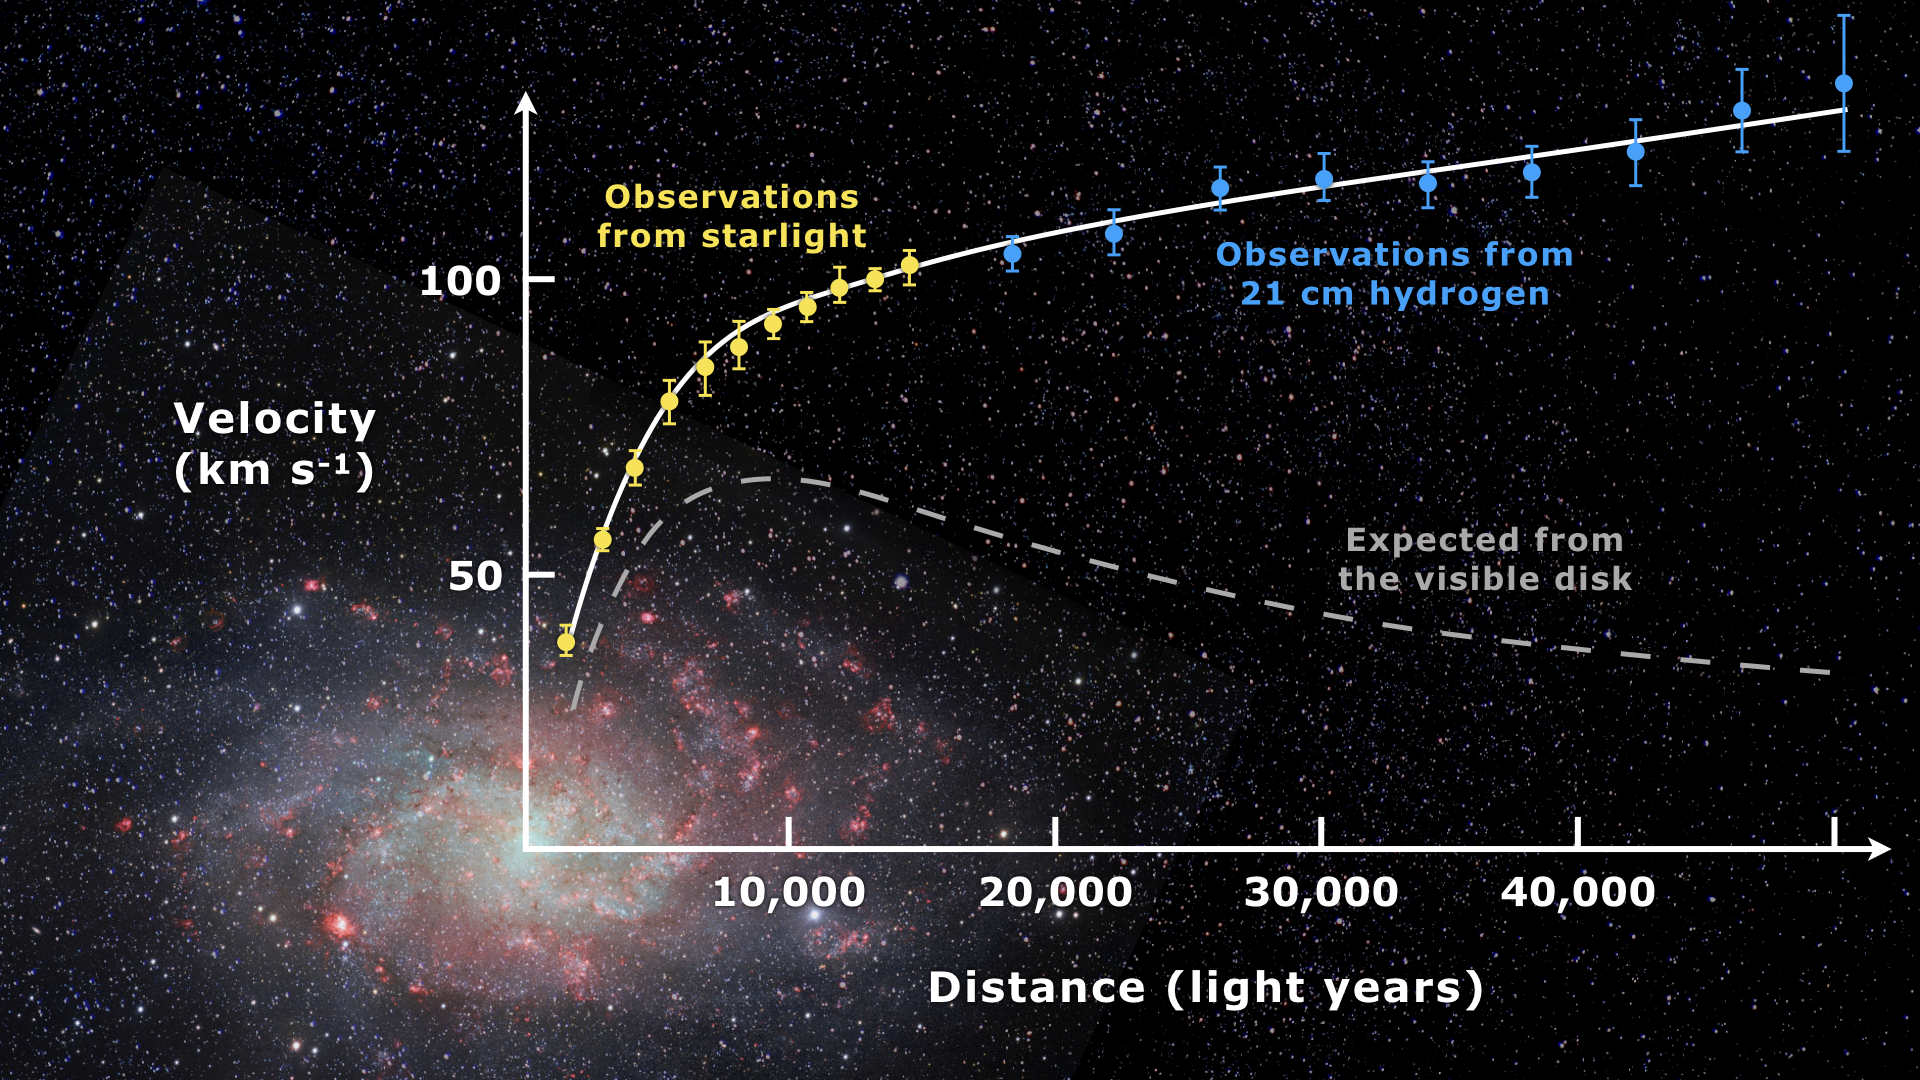
\includegraphics[width=0.9\textwidth,clip=]{thesis_template_cua/Figures/CH2_DM/galac_curve.png}
         \vspace*{10mm}
         \caption[Galactic Rotation Curve]{This figure depicts the rotational curve of spiral galaxy Messier 33 (yellow and blue points with error bars), and a predicted one from distribution of the visible matter (gray line). The discrepancy between the two curves can be accounted for by adding a dark matter halo surrounding the galaxy.}
         \label{ch2:rot_curve}
\end{figure}

\begin{figure} [tpb]
\centering
         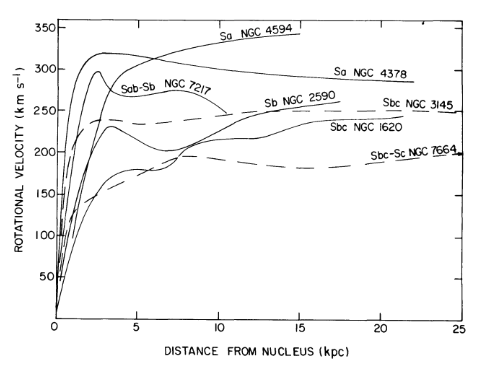
\includegraphics[width=0.9\textwidth,clip=]{thesis_template_cua/Figures/CH2_DM/many_rot_curve.png}
         \vspace*{10mm}
         \caption[Galactic Rotation Curves]{This figure depicts the rotational curves of many galaxies as observed by \citep{CH2_DM:rot_curves}. The flat tail characteristic at large distance is very much evident}
         \label{ch2:rot_curves}
\end{figure}

From Figure \ref{ch2:core_cusp} we can see that observations clearly indicate approximately constant dark matter density in the inner parts of the galaxies, while the cosmological numerical simulations indicate a steep power-law like distribution. This deviation in the theoretical predictions is referred to as the $"core-cusp"$ problem \citep{ch2:core-cusp}.
However, the dark matter scientific community seems to have opinions on the reasons for the $"core-cusp"$ problem arising either from incomplete understanding of galaxy core dynamics or experimental limitations in the measurements.

Be that as it may, we can say that dark matter is necessary for the explanation of the velocities in the galactic rotation curves.


\begin{figure} [tpb]
\centering
         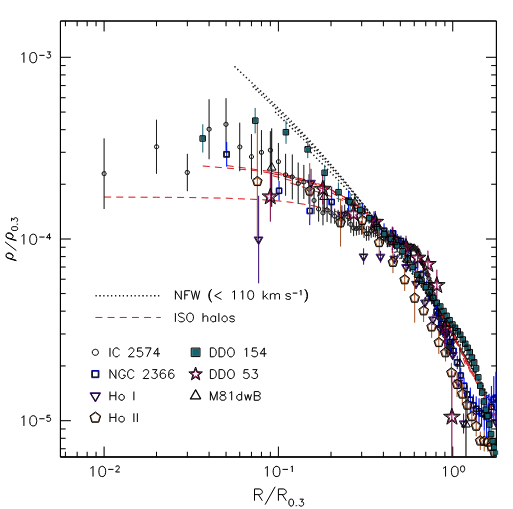
\includegraphics[width=0.65\textwidth,clip=]{thesis_template_cua/Figures/CH2_DM/core-cusp.png}
         \vspace*{10mm}
         \caption[Core Cusp density Profile]{This figure depicts the dark matter density profiles of seven dwarf galaxies indicated by the data points and the theoretical prediction model indicated by the black dotted lines. The deviation of the observations from the theoretical predictions as we move to the center of the galaxy is referred as the "core-cusp" problem. }
         \label{ch2:core_cusp}
\end{figure}
%Maybe a sentence or two that bring the argument and evidence together.\citep{dos_santos_2020}

% \begin{table}[h!]
%   \centering
%   \caption{Very important table.}
%   \label{tab:average_channels}
%   \begin{tabular}{cc}
%     \toprule
%      AIA channel (\AA) &  Scaling unit [DN/s/pixel] \\
%      \midrule
%       94 &   10  \\
%       131 &   80  \\
%       171 & 2000  \\
%       193 & 3000  \\
%       211 & 1000  \\
%       304 &  500  \\
%       335 &   80  \\
%       \bottomrule
%   \end{tabular}
% \end{table}

\subsection{Gravitational Lensing}
The phenomenon of gravitational lensing is the bending of light when it travels near massive objects like the sun in analogy with the bending of light through a lens. It is a consequence of Einstein's General theory of Relativity \citep{ch2:relativity} which states that the path of the light is bent by gravity when it travels close to a massive object like the sun. This phenomenon was experimentally observed by Arthur Eddington and Andrew Claude Crommelin and Charles Davidson separately at the island of Principe (West Africa) and Sobral (Brazil). They measured the position of a bright group of stars called Haydes, which at the time of the eclipse were behind the sun and were easier to observe because of their brightness. After analysing the photographs it was observed that the stars behind the sun were indeed visible confirming the Einstein's theory of the curvature of the space-time and the phenomenon of gravitational lensing.

Gravitational lensing has been the most successful technique to investigate dark matter. The deflection of the rays of light by this phenomena creates effects such as shifting, distorting and magnifying the images of background galaxies, as shown in figure \ref{ch2:grav_lensing}. Probing such effects has provided constraints on the properties of dark matter such as mass, mean density relative to matter and size \citep{ch2:lensing}. 

\begin{figure} [tpb]
\centering
         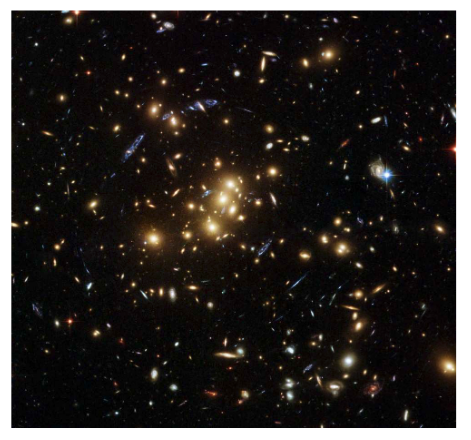
\includegraphics[width=0.5\textwidth,clip=]{thesis_template_cua/Figures/CH2_DM/lensing.png}
         \vspace*{10mm}
         \caption[Gravitational Lensing]{This figure shows the effect of gravitational lensing around the galaxy cluster CL0024+17. The elongated blue objects are physically unassociated galaxies lying behind the cluster and appear as tangential arcs. They appear to be distorted because of the gravitational lensing effects. (Figure credit:NASA/ESA/M.J. Jee (John Hopkins University)) }
         \label{ch2:grav_lensing}
\end{figure}
The assembly of galaxy clusters involves complex physical processes, these processes affect the baryonic mass and the dark matter differently, thus distorting the distributions of baryonic mass and the dark matter.Galaxy clusters contain three basic ingredients: galaxies, intra-cluster gas and dark matter. The "bullet cluster", a two cluster setup that collided about 150 years ago \citep{ch2:bullet1, ch2:bullet2} has provided the most direct evidence for the effect of these processes as shown in the left image of Figure \ref{ch2:bullet_cluster} indicating that the ingredients have separated. Similar to particle production at a particle collider, the trajectories of the cluster debris are also governed by the properties of its constituents. 
\begin{figure} [tpb]
\centering
         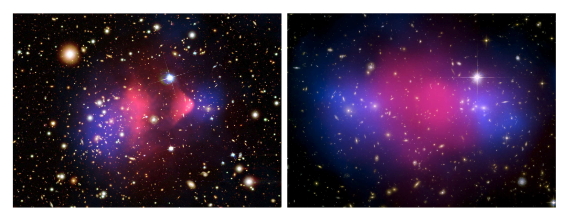
\includegraphics[width=0.9\textwidth,clip=]{thesis_template_cua/Figures/CH2_DM/bullet_cluster.png}
         \vspace*{10mm}
         \caption[Bullet Cluster]{This figure shows the
observed X-ray emission from hot intra-cluster gas due to plasma in galaxy cluster merger 1E0657-558,
also known as the Bullet Cluster \citep{ch2:bullet2}. The striking discrepancy between the inferred dark
matter and observed plasma distributions in this merger providing a strong evidence for the existence of an additional reserve of dark matter. (Figure credit:
Left: X-ray: NASA/CXC/CfA/ M.Markevitch et al.; Lensing Map: NASA/STScI;
ESO WFI; Magellan/U.Arizona/ D.Clowe et al. Optical image: NASA/STScI;
Magellan/U.Arizona/D.Clowe et al.; Right: NASA/ESA/M.Bradac et al.). }
         \label{ch2:bullet_cluster}
\end{figure}

Since individual galaxies inside the cluster are well spaced meaning that, they have very low collisional cross-section, implying their continued movement during the collision far from the point of impact. While the intra-cluster gas is uniformly spread and has a large collisional cross-section, thus slowing it down. One may think that all the mass in the cluster can be defined by the above two ingredients, but a significant of amount of mass is observed to be located near the galaxies. For the mass to have travelled this distance it must have some sort of self-interaction collisional cross-section. And gravitational lensing observations require the third ingredient of the bullet cluster which is the dark matter to explain the above effect.

\subsection{Dark Matter Seeded Galaxy formations}

More ideas that really make this a great paper. Maybe a footnote or two.\footnote{Some peripheral thoughts that belong in a note.}
